\documentclass[14pt]{extbook}
\usepackage{multicol, enumerate, enumitem, hyperref, color, soul, setspace, parskip, fancyhdr} %General Packages
\usepackage{amssymb, amsthm, amsmath, bbm, latexsym, units, mathtools} %Math Packages
\everymath{\displaystyle} %All math in Display Style
% Packages with additional options
\usepackage[headsep=0.5cm,headheight=12pt, left=1 in,right= 1 in,top= 1 in,bottom= 1 in]{geometry}
\usepackage[usenames,dvipsnames]{xcolor}
\usepackage{dashrule}  % Package to use the command below to create lines between items
\newcommand{\litem}[1]{\item#1\hspace*{-1cm}\rule{\textwidth}{0.4pt}}
\pagestyle{fancy}
\lhead{Progress Quiz 4}
\chead{}
\rhead{Version C}
\lfoot{6286-1986}
\cfoot{}
\rfoot{Fall 2020}
\begin{document}

\begin{enumerate}
\litem{
Choose the graph of the equation below.\[ f(x) = \frac{-1}{(x + 3)^2} - 1 \]\begin{enumerate}[label=\Alph*.]
\begin{multicols}{2}\item 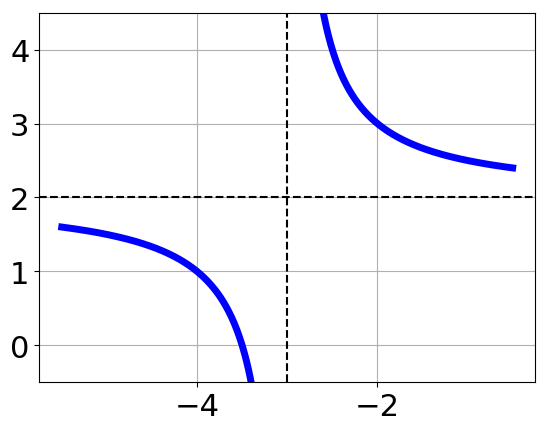
\includegraphics[width = 0.3\textwidth]{../Figures/rationalEquationToGraphAC.png}\item 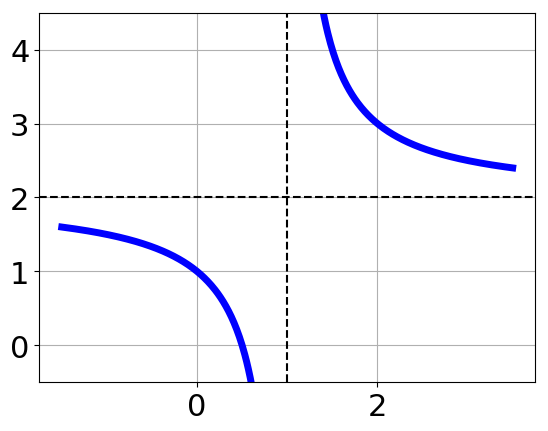
\includegraphics[width = 0.3\textwidth]{../Figures/rationalEquationToGraphBC.png}\item 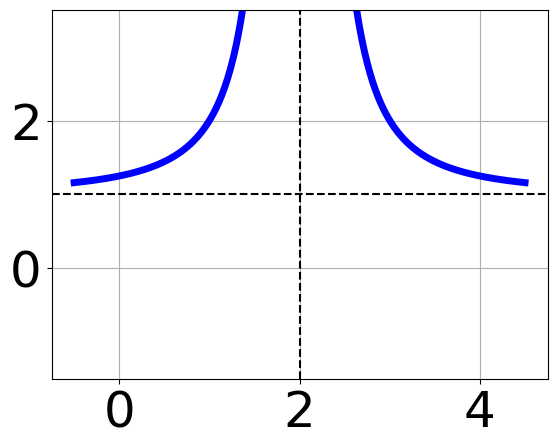
\includegraphics[width = 0.3\textwidth]{../Figures/rationalEquationToGraphCC.png}\item 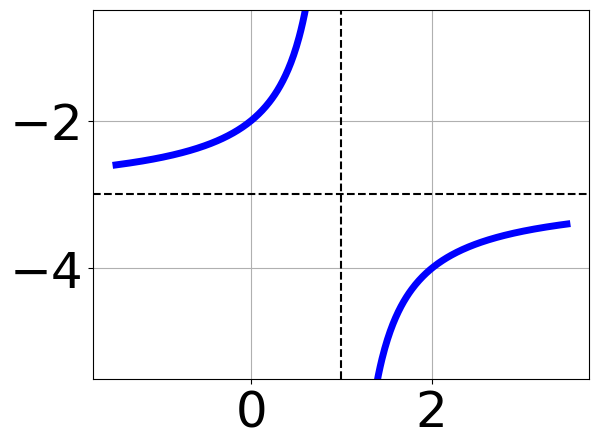
\includegraphics[width = 0.3\textwidth]{../Figures/rationalEquationToGraphDC.png}\end{multicols}\item None of the above.
\end{enumerate} }
\litem{
Choose the equation of the function graphed below.
\begin{center}
    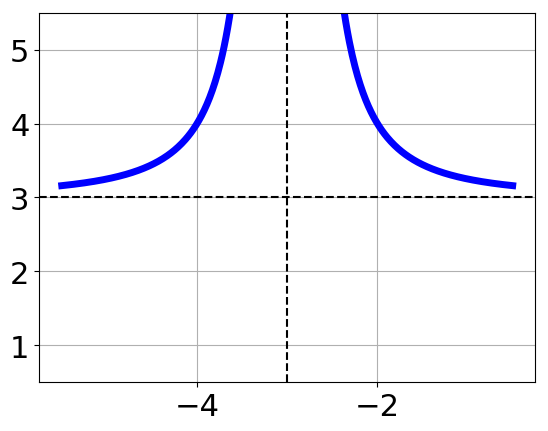
\includegraphics[width=0.5\textwidth]{../Figures/rationalGraphToEquationC.png}
\end{center}
\begin{enumerate}[label=\Alph*.]
\item \( f(x) = \frac{1}{x + 3} - 2 \)
\item \( f(x) = \frac{-1}{x - 3} - 2 \)
\item \( f(x) = \frac{-1}{(x - 3)^2} - 2 \)
\item \( f(x) = \frac{1}{(x + 3)^2} - 2 \)
\item \( \text{None of the above} \)

\end{enumerate} }
\litem{
Solve the rational equation below. Then, choose the interval(s) that the solution(s) belongs to.\[ \frac{7}{4x -4} + 2 = \frac{-5}{-16x + 16} \]\begin{enumerate}[label=\Alph*.]
\item \( \text{All solutions lead to invalid or complex values in the equation.} \)
\item \( x \in [0.28,1.28] \)
\item \( x_1 \in [-2.8, -1.1] \text{ and } x_2 \in [-0.72,2.28] \)
\item \( x_1 \in [-0.8, -0.3] \text{ and } x_2 \in [-0.72,2.28] \)
\item \( x \in [-2.8,-1.1] \)

\end{enumerate} }
\litem{
Determine the domain of the function below.\[ f(x) = \frac{3}{25x^{2} +40 x + 15} \]\begin{enumerate}[label=\Alph*.]
\item \( \text{All Real numbers except } x = a \text{ and } x = b, \text{ where } a \in [-1.87, -0.79] \text{ and } b \in [-0.87, -0.22] \)
\item \( \text{All Real numbers.} \)
\item \( \text{All Real numbers except } x = a, \text{ where } a \in [-25.39, -24.25] \)
\item \( \text{All Real numbers except } x = a \text{ and } x = b, \text{ where } a \in [-25.39, -24.25] \text{ and } b \in [-15.38, -14.04] \)
\item \( \text{All Real numbers except } x = a, \text{ where } a \in [-1.87, -0.79] \)

\end{enumerate} }
\litem{
Solve the rational equation below. Then, choose the interval(s) that the solution(s) belongs to.\[ \frac{2x}{-5x + 2} + \frac{-2x^{2}}{-35x^{2} +44 x -12} = \frac{-3}{7x -6} \]\begin{enumerate}[label=\Alph*.]
\item \( x_1 \in [0.25, 0.38] \text{ and } x_2 \in [-1.6,1.4] \)
\item \( \text{All solutions lead to invalid or complex values in the equation.} \)
\item \( x \in [0.57,0.86] \)
\item \( x_1 \in [0.25, 0.38] \text{ and } x_2 \in [2,6] \)
\item \( x \in [1.49,2.35] \)

\end{enumerate} }
\litem{
Choose the equation of the function graphed below.
\begin{center}
    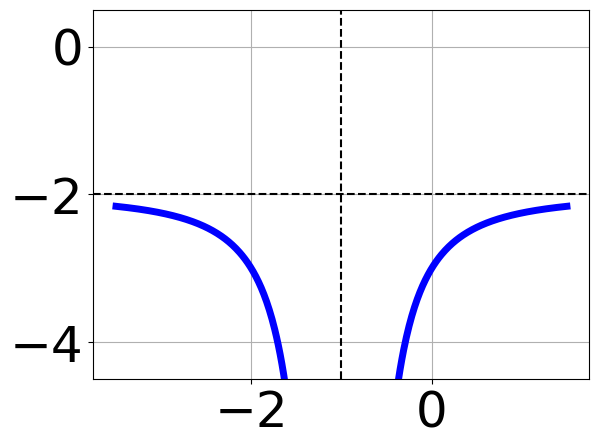
\includegraphics[width=0.5\textwidth]{../Figures/rationalGraphToEquationCopyC.png}
\end{center}
\begin{enumerate}[label=\Alph*.]
\item \( f(x) = \frac{-1}{(x + 2)^2} + 1 \)
\item \( f(x) = \frac{1}{x - 2} + 1 \)
\item \( f(x) = \frac{-1}{x + 2} + 1 \)
\item \( f(x) = \frac{1}{(x - 2)^2} + 1 \)
\item \( \text{None of the above} \)

\end{enumerate} }
\litem{
Choose the graph of the equation below.\[ f(x) = \frac{1}{x + 2} - 3 \]\begin{enumerate}[label=\Alph*.]
\begin{multicols}{2}\item 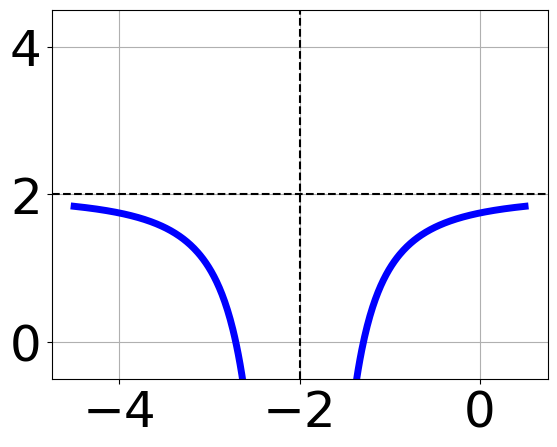
\includegraphics[width = 0.3\textwidth]{../Figures/rationalEquationToGraphCopyAC.png}\item 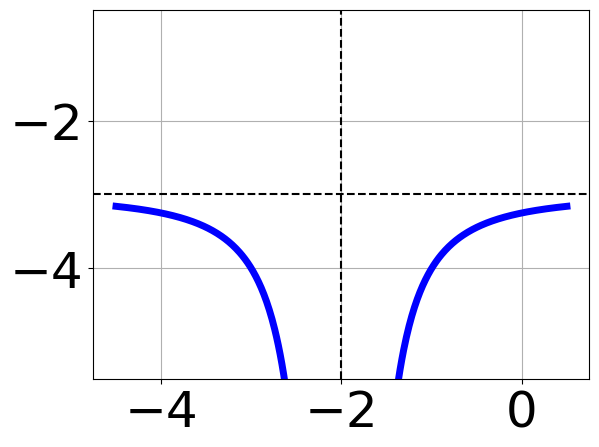
\includegraphics[width = 0.3\textwidth]{../Figures/rationalEquationToGraphCopyBC.png}\item 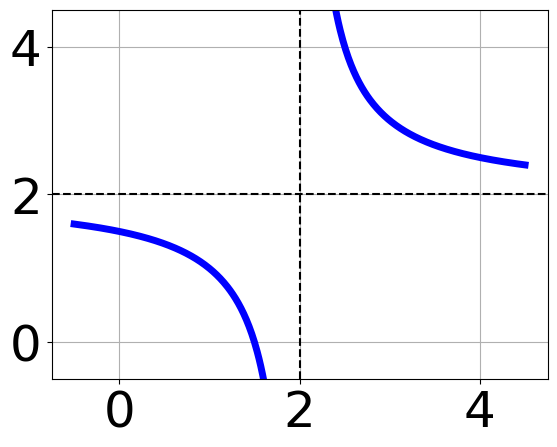
\includegraphics[width = 0.3\textwidth]{../Figures/rationalEquationToGraphCopyCC.png}\item 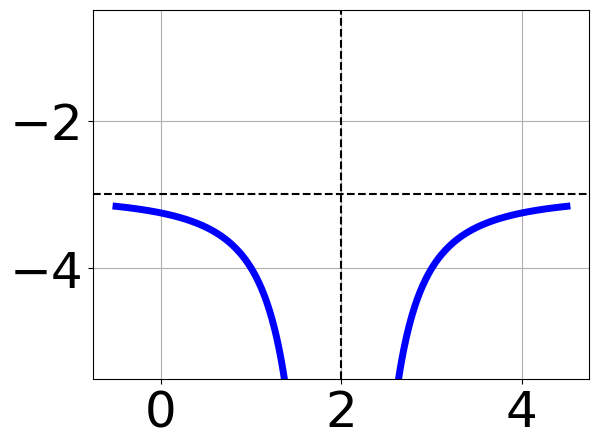
\includegraphics[width = 0.3\textwidth]{../Figures/rationalEquationToGraphCopyDC.png}\end{multicols}\item None of the above.
\end{enumerate} }
\litem{
Solve the rational equation below. Then, choose the interval(s) that the solution(s) belongs to.\[ \frac{9}{-6x + 4} + -9 = \frac{-3}{-54x + 36} \]\begin{enumerate}[label=\Alph*.]
\item \( x_1 \in [0.39, 0.47] \text{ and } x_2 \in [0.49,1.49] \)
\item \( x_1 \in [-0.87, -0.82] \text{ and } x_2 \in [0.49,1.49] \)
\item \( x \in [0.49,1.49] \)
\item \( x \in [-0.87,-0.82] \)
\item \( \text{All solutions lead to invalid or complex values in the equation.} \)

\end{enumerate} }
\litem{
Solve the rational equation below. Then, choose the interval(s) that the solution(s) belongs to.\[ \frac{5x}{-2x -3} + \frac{-2x^{2}}{-8x^{2} -2 x + 15} = \frac{-5}{4x -5} \]\begin{enumerate}[label=\Alph*.]
\item \( \text{All solutions lead to invalid or complex values in the equation.} \)
\item \( x \in [0.58,1.76] \)
\item \( x_1 \in [-0.99, -0.09] \text{ and } x_2 \in [-2.5,0.5] \)
\item \( x \in [1.75,2.45] \)
\item \( x_1 \in [-0.99, -0.09] \text{ and } x_2 \in [0.31,6.31] \)

\end{enumerate} }
\litem{
Determine the domain of the function below.\[ f(x) = \frac{6}{30x^{2} -11 x -30} \]\begin{enumerate}[label=\Alph*.]
\item \( \text{All Real numbers except } x = a \text{ and } x = b, \text{ where } a \in [-4.83, 0.17] \text{ and } b \in [-0.8, 2.2] \)
\item \( \text{All Real numbers except } x = a \text{ and } x = b, \text{ where } a \in [-33, -29] \text{ and } b \in [30, 31] \)
\item \( \text{All Real numbers except } x = a, \text{ where } a \in [-4.83, 0.17] \)
\item \( \text{All Real numbers.} \)
\item \( \text{All Real numbers except } x = a, \text{ where } a \in [-33, -29] \)

\end{enumerate} }
\end{enumerate}

\end{document}